%% Guilherme N. Ramos (gnramos@unb.br)
%% Baseado em https://www.urionlinejudge.com.br/judge/en/problems/view/1168

\NomeDoProblema{LED}%
\Conceitos{Ad-Hoc,string}%
\Dificuldade{1}%

Um \emph{diodo emissor de luz} (LED) pode ser usado como uma lâmpada extremamente
eficiente e Tio Ernie que utilizá-los para montar o placar em seu novíssimo estádio
para Competições de Pinball. Ele sabe que Tommy, atual campeão da competição deve
inaugurar o placar, e precisa saber quantos LEDs vai precisar para mostrar a
pontuação dos competidores.

Considerando a configuração de LEDs dos números abaixo (cada traço é um LED),
faça um algoritmo que ajude Tio Ernie a descobrir o número de LEDs necessário
para exibir tal valor.

\begin{center}
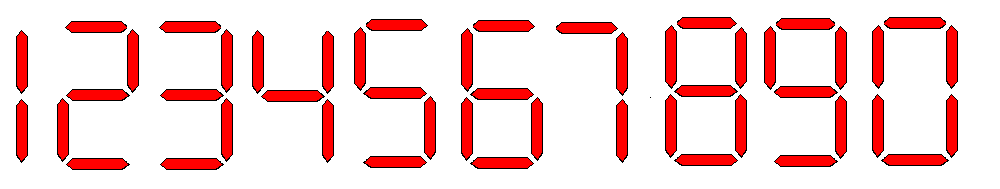
\includegraphics[width=.8\textwidth]{leds}%
\end{center}%

\subsection*{Entrada}%
A entrada contém um inteiro $N$, $(1 \leq N \leq 10^{100})$, correspondendo a
pontuação do competidor.

\subsection*{Saída}%
Mostre uma linha contendo o número de LEDs que Tio Ernie precisará para exibir a
pontuação, seguido pela palavra ``LEDs'' (e quebra de linha!).

\Exemplos{1,13}%